% The prism operator: split Delta^1 x [0,1] into triangles, push via sigma x id then F into Y.
% Source: book/tex/homology/singular.tex (§ Geometry of chain complexes).
\documentclass[border=2mm]{standalone}
\usepackage{tikz}
\usepackage{amsmath}
\usetikzlibrary{arrows.meta}
\definecolor{heavygreen}{rgb}{0,0.5,0}
\begin{document}
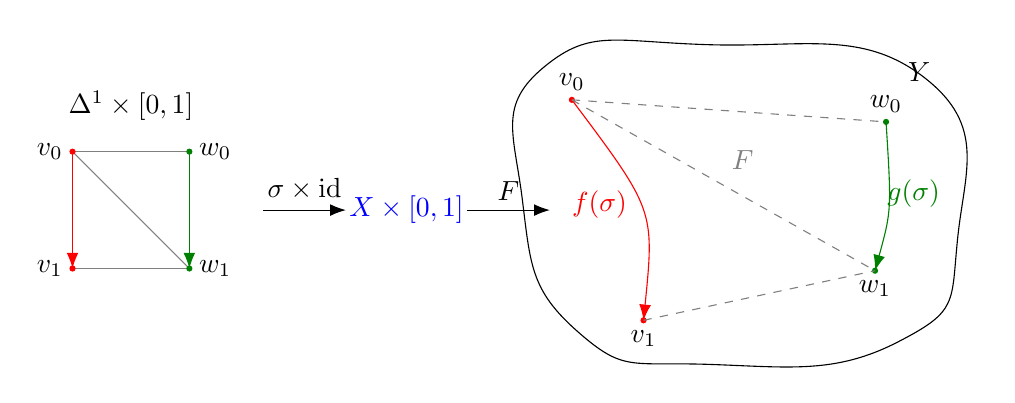
\begin{tikzpicture}[>={Latex[length=2mm]}, scale=0.7]
  % Left: Delta^1 x [0,1] square
  \coordinate (W) at (-1.06,1.06); \coordinate (Xc) at (-1.06,-1.06);
  \coordinate (Yc) at (1.06,1.06); \coordinate (Z) at (1.06,-1.06);
  \node at (0,1.9) {$\Delta^1 \times [0,1]$};
  \draw[red, ->] (W)--(Xc);
  \draw[heavygreen, ->] (Yc)--(Z);
  \draw[gray] (W)--(Yc); \draw[gray] (Xc)--(Z); \draw[gray] (W)--(Z);
  \fill[red] (W) circle (1.6pt) node[left,black]{$v_0$};
  \fill[red] (Xc) circle (1.6pt) node[left,black]{$v_1$};
  \fill[heavygreen] (Yc) circle (1.6pt) node[right,black]{$w_0$};
  \fill[heavygreen] (Z) circle (1.6pt) node[right,black]{$w_1$};
  % middle arrows
  \draw[->] (2.4,0)--(3.9,0) node[midway,above]{$\sigma \times \operatorname{id}$};
  \node[blue] at (5,0) {$X \times [0,1]$};
  \draw[->] (6.1,0)--(7.6,0) node[midway,above]{$F$};
  % Right: Y blob with deformed 1-simplex
  \begin{scope}[shift={(11.5,0)}]
    \draw plot[smooth cycle, tension=0.9]
      coordinates {(-4,2.6)(-1,3)(2.9,2.4)(3.5,-0.5)(2.4,-2.4)(-1,-2.8)(-3.4,-2.2)(-4.4,0.2)};
    \node at (2.8,2.5) {$Y$};
    \coordinate (A) at (-3.5,2); \coordinate (B) at (-2.2,-2);
    \coordinate (C) at (2.2,1.6); \coordinate (D) at (2,-1.1);
    \draw[red, ->] (A) .. controls (-2,0) .. (B);
    \fill[red] (A) circle (1.6pt) node[above,black]{$v_0$};
    \fill[red] (B) circle (1.6pt) node[below,black]{$v_1$};
    \node[red] at (-3,0.1) {$f(\sigma)$};
    \draw[heavygreen, ->] (C) .. controls (2.3,0) .. (D);
    \fill[heavygreen] (C) circle (1.6pt) node[above,black]{$w_0$};
    \fill[heavygreen] (D) circle (1.6pt) node[below,black]{$w_1$};
    \node[heavygreen] at (2.7,0.3) {$g(\sigma)$};
    \draw[gray, dashed] (A)--(C);
    \draw[gray, dashed] (A)--(D);
    \node[gray] at (-0.4,0.9) {$F$};
    \draw[gray, dashed] (B)--(D);
  \end{scope}
\end{tikzpicture}
\end{document}
